 \documentclass[12pt,letterpaper]{article}
\usepackage[margin=0.9 in]{geometry}
\setlength{\parskip}{\baselineskip}%
\setlength{\parindent}{20pt}%
\usepackage{setspace}
% \singlespacing
% \onehalfspacing
% \doublespacing
% \setstretch{<factor>} % for custom spacing
\setstretch{1.5}
% reduce space between equations:
\AtBeginDocument{%
  \addtolength\abovedisplayskip{-0.2\baselineskip}%
  \addtolength\belowdisplayskip{-0.2\baselineskip}%
%  \addtolength\abovedisplayshortskip{-0.5\baselineskip}%
%  \addtolength\belowdisplayshortskip{-0.5\baselineskip}%
}

\usepackage[toc,page]{appendix}

\usepackage[colorlinks=true,
            linkcolor=red,
            urlcolor=blue,
            citecolor=red]{hyperref}

\usepackage[toc,page]{appendix}
\usepackage{pdflscape}
\usepackage[english]{babel}
\usepackage[utf8x]{inputenc}
\usepackage{amsmath}
\usepackage{amsthm}
    \newtheorem{thm}{\protect\theoremname}
    \theoremstyle{plain}
    \newtheorem{prop}[thm]{\protect\propositionname}
    \theoremstyle{plain}
    \newtheorem{assumption}[thm]{\protect\assumptionname}
    \providecommand{\assumptionname}{Assumption}
    \providecommand{\propositionname}{Proposition}
    \providecommand{\theoremname}{Theorem}

    \theoremstyle{definition}
    \newtheorem{defn}{Definition}[section]
    \newtheorem{conj}{Conjecture}[section]
    \newtheorem{exmp}{Example}[section]
    \theoremstyle{remark}
    \newtheorem*{rem}{Remark}
    \newtheorem*{note}{Note}
\usepackage{amssymb} 
\usepackage[retainorgcmds]{IEEEtrantools}
\usepackage{graphicx}
\usepackage{tabularx}
\usepackage{subfig}
\usepackage{kpfonts}    % for nice fonts
\usepackage{microtype} 
\usepackage{booktabs}   % for nice tables
\usepackage{bm}         % for bold math
\usepackage{listings}   % for inserting code
\usepackage{verbatim}   % useful for program listings
\usepackage{color}  
\usepackage[colorlinks=true]{hyperref}
% use for hypertext
\usepackage[font={small,it}]{caption}
\usepackage{natbib}
\usepackage{cleveref}
% Need the following to render tables:
\usepackage{dcolumn}
\usepackage{rotating}
\usepackage{geometry}
\usepackage{pdflscape}
\usepackage{bbm}
\usepackage{threeparttable}

% \usepackage[colorinlistoftodos]{todonotes}
\usepackage{xargs} % Use more than one optional parameter in a new commands
\usepackage[pdftex,dvipsnames]{xcolor}  % Coloured text etc.
 
% to DISABLE todo notes add disable into the options list.
% \usepackage[colorinlistoftodos,prependcaption,textsize=tiny, disable]{todonotes}
\usepackage[colorinlistoftodos,prependcaption,textsize=tiny]{todonotes}
\newcommandx{\unsure}[2][1=]{\todo[linecolor=red,backgroundcolor=red!25,bordercolor=red,#1]{#2}}
\newcommandx{\change}[2][1=]{\todo[linecolor=blue,backgroundcolor=blue!25,bordercolor=blue,#1]{#2}}
\newcommandx{\info}[2][1=]{\todo[linecolor=OliveGreen,backgroundcolor=OliveGreen!25,bordercolor=OliveGreen,#1]{#2}}
\newcommandx{\improvement}[2][1=]{\todo[linecolor=Plum,backgroundcolor=Plum!25,bordercolor=Plum,#1]{#2}}
\newcommandx{\thiswillnotshow}[2][1=]{\todo[disable,#1]{#2}}

\usepackage[section]{placeins} %This prevents placing floats before a section.

%========================================================================


\begin{document}


\begin{figure}[h!]
    \centering
    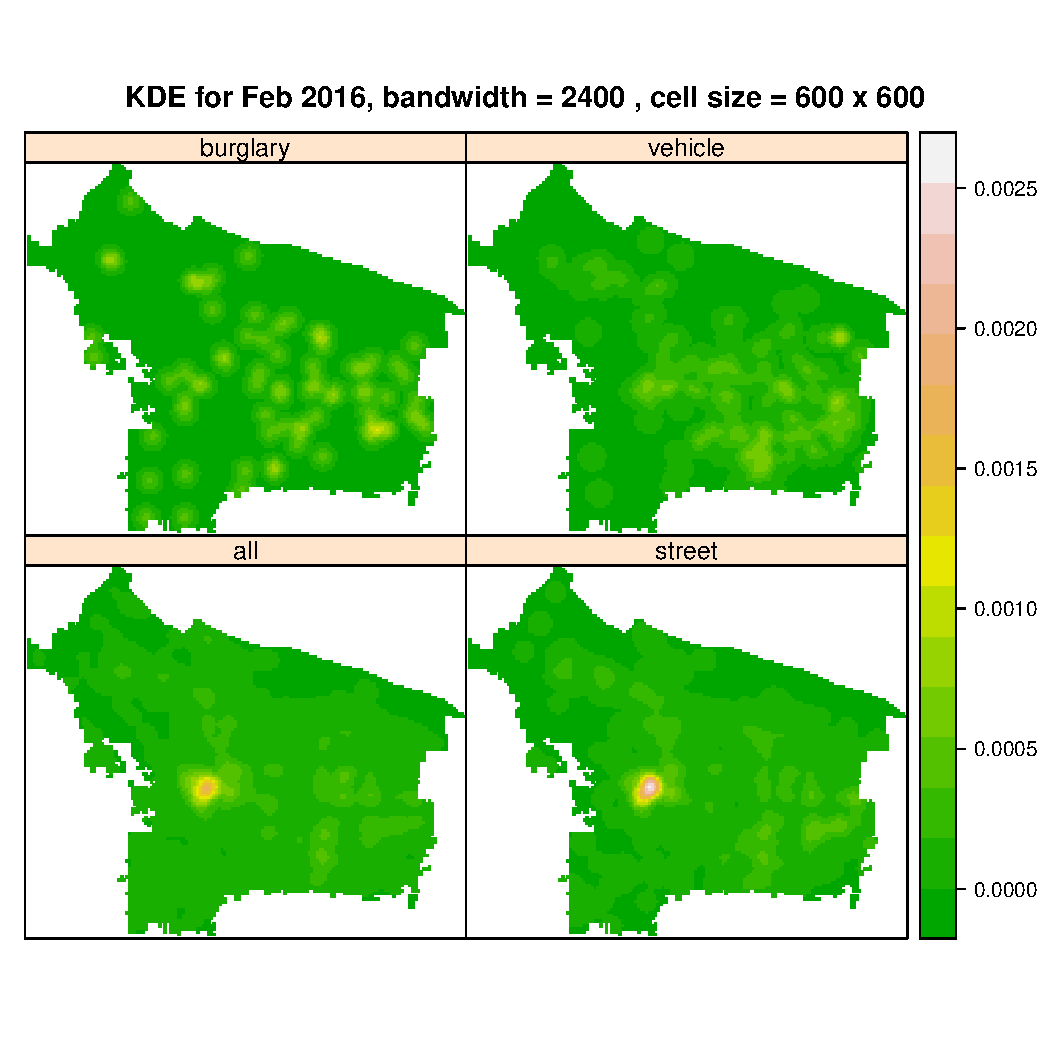
\includegraphics[]{figures/kde_bycategory.pdf}
    \caption{}
    \label{fig:figure1}
\end{figure}


\begin{figure}[h!]
    \centering
    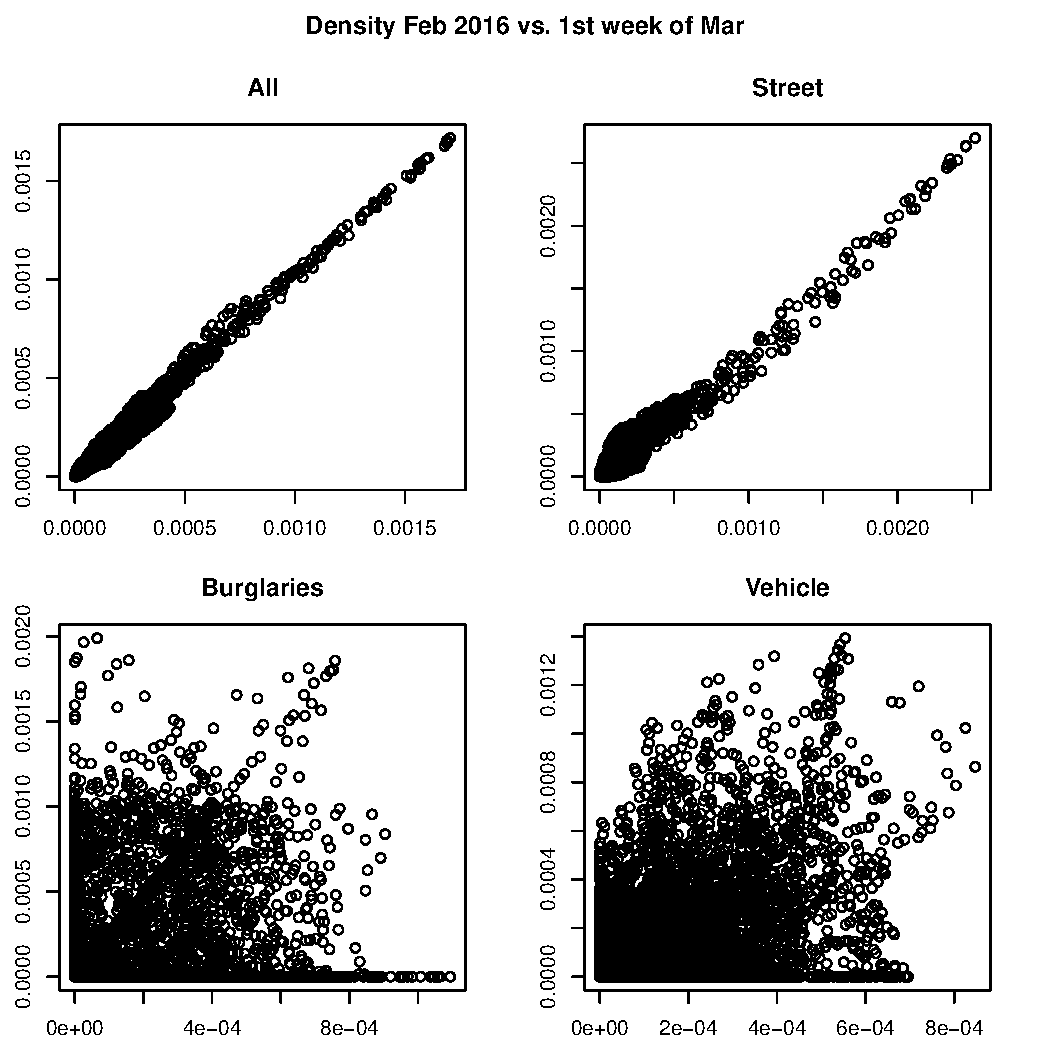
\includegraphics[]{figures/scatter_kde_1w.pdf}
    \caption{Scatter plots of the KDE of each cell. In the x-axis: KDE for Feb 2016.}
    \label{fig:figure1}
\end{figure}

\begin{figure}[h!]
    \centering
    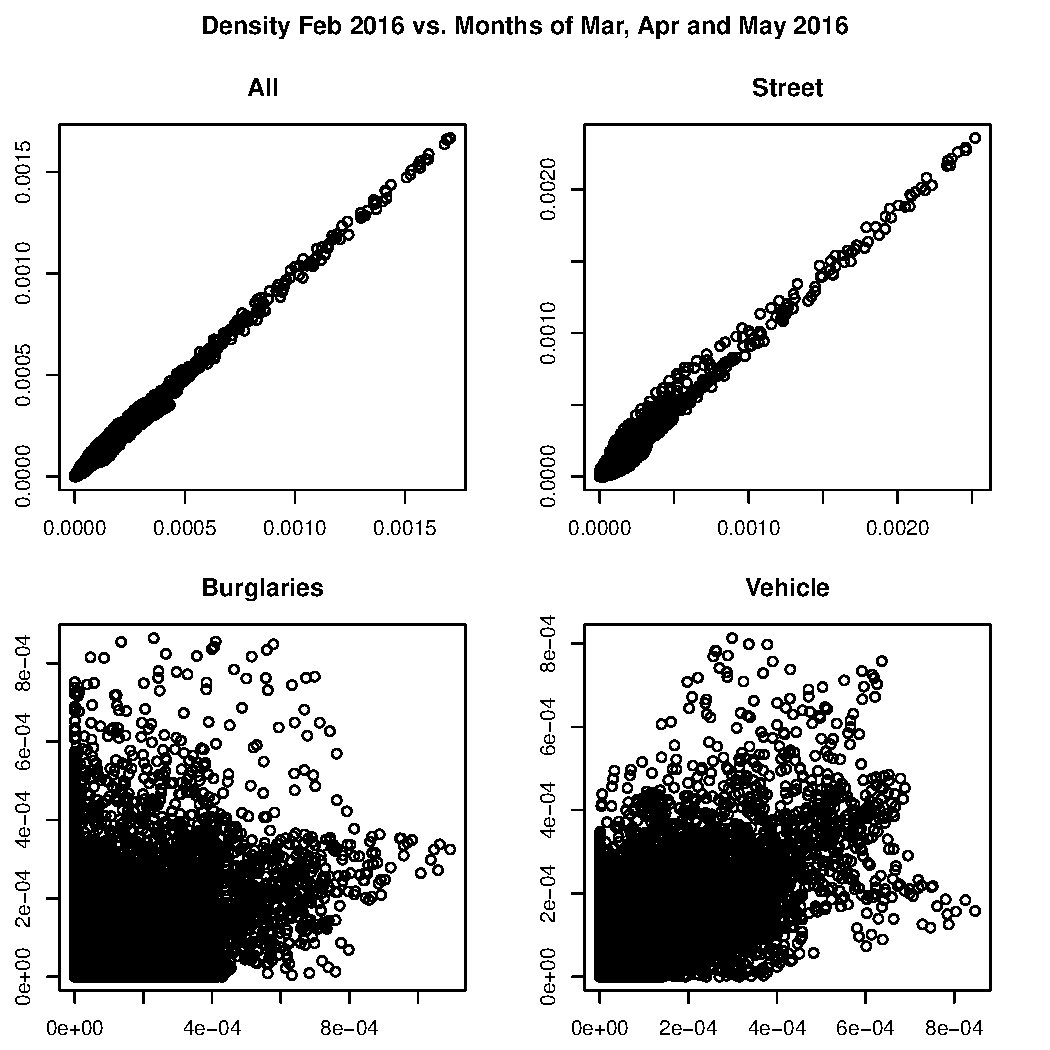
\includegraphics[]{figures/scatter_kde_3m.pdf}
    \caption{Scatter plots of the KDE of each cell. In the x-axis: KDE for Feb 2016.}
    \label{fig:figure1}
\end{figure}

\begin{table}[h!]
    \centering
    \caption{Spearman Rank Correlations}
    \begin{threeparttable}
        
% Table created by stargazer v.5.2 by Marek Hlavac, Harvard University. E-mail: hlavac at fas.harvard.edu
% Date and time: Tue, Oct 25, 2016 - 08:03:24 PM
\begin{tabular}{@{\extracolsep{5pt}} ccccc} 
\\[-1.8ex]\hline 
\hline \\[-1.8ex] 
 & all & street & burglary & vehicle \\ 
\hline \\[-1.8ex] 
w1 & $0.986$ & $0.931$ & $0.356$ & $0.676$ \\ 
w2 & $0.989$ & $0.941$ & $0.421$ & $0.723$ \\ 
m1 & $0.990$ & $0.947$ & $0.466$ & $0.747$ \\ 
m2 & $0.981$ & $0.928$ & $0.403$ & $0.595$ \\ 
m3 & $0.984$ & $0.924$ & $0.404$ & $0.684$ \\ 
\hline \\[-1.8ex] 
\end{tabular} 
 
        \begin{tablenotes}\footnotesize
        \item[*] Spearman rank correlations computed from the KDE estimates for different crime categories, using a grid with cell size of 600x600 squared feet.
        \end{tablenotes}
    \end{threeparttable}
\end{table}

\begin{figure}[h!]
    \centering
    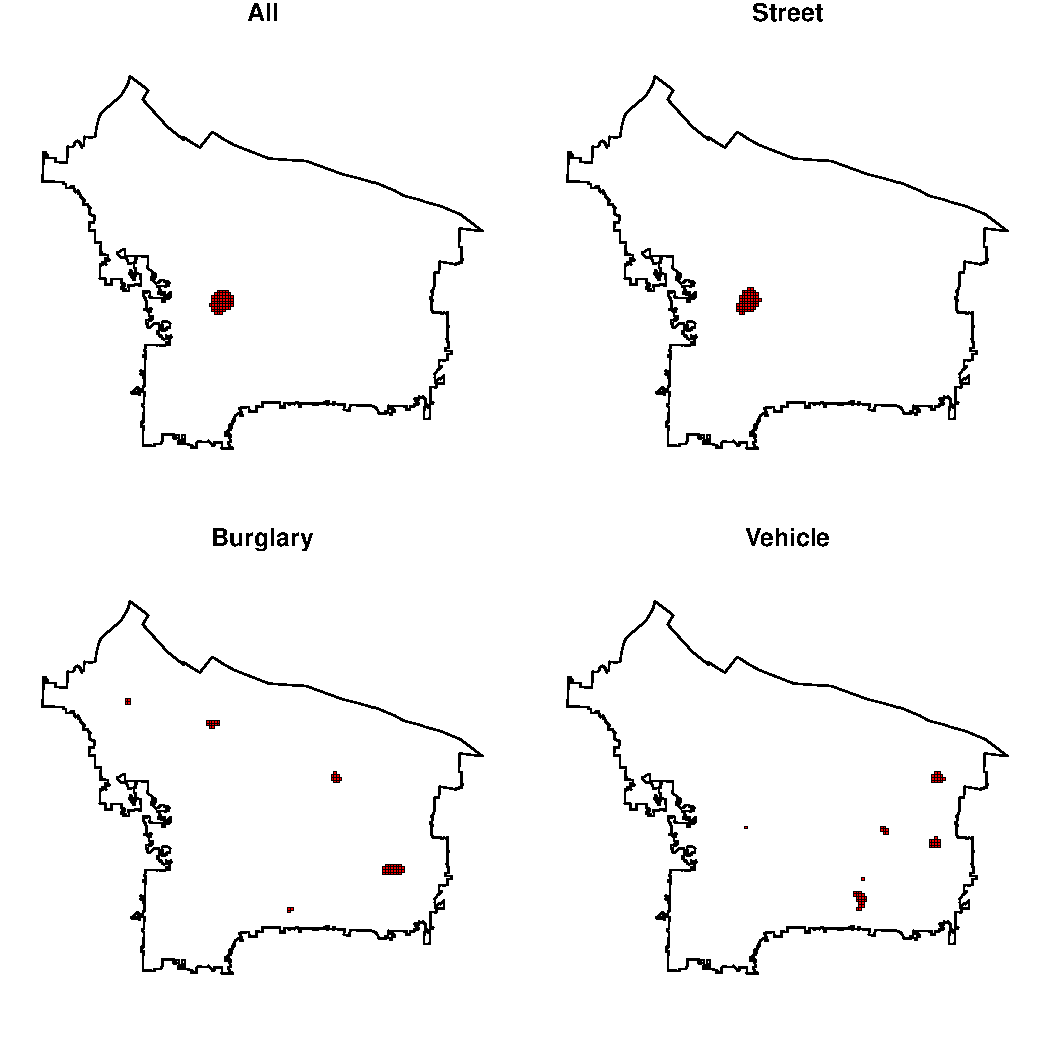
\includegraphics[]{figures/max_areas.pdf}
    \caption{Selection of the highest denisty cells for each crime category. The maximum forecasted area using cell sizes of 600x600 feet is encompassed by 58 cells.}
    \label{fig:figure1}
\end{figure}


\begin{figure}[h!]
    \centering
    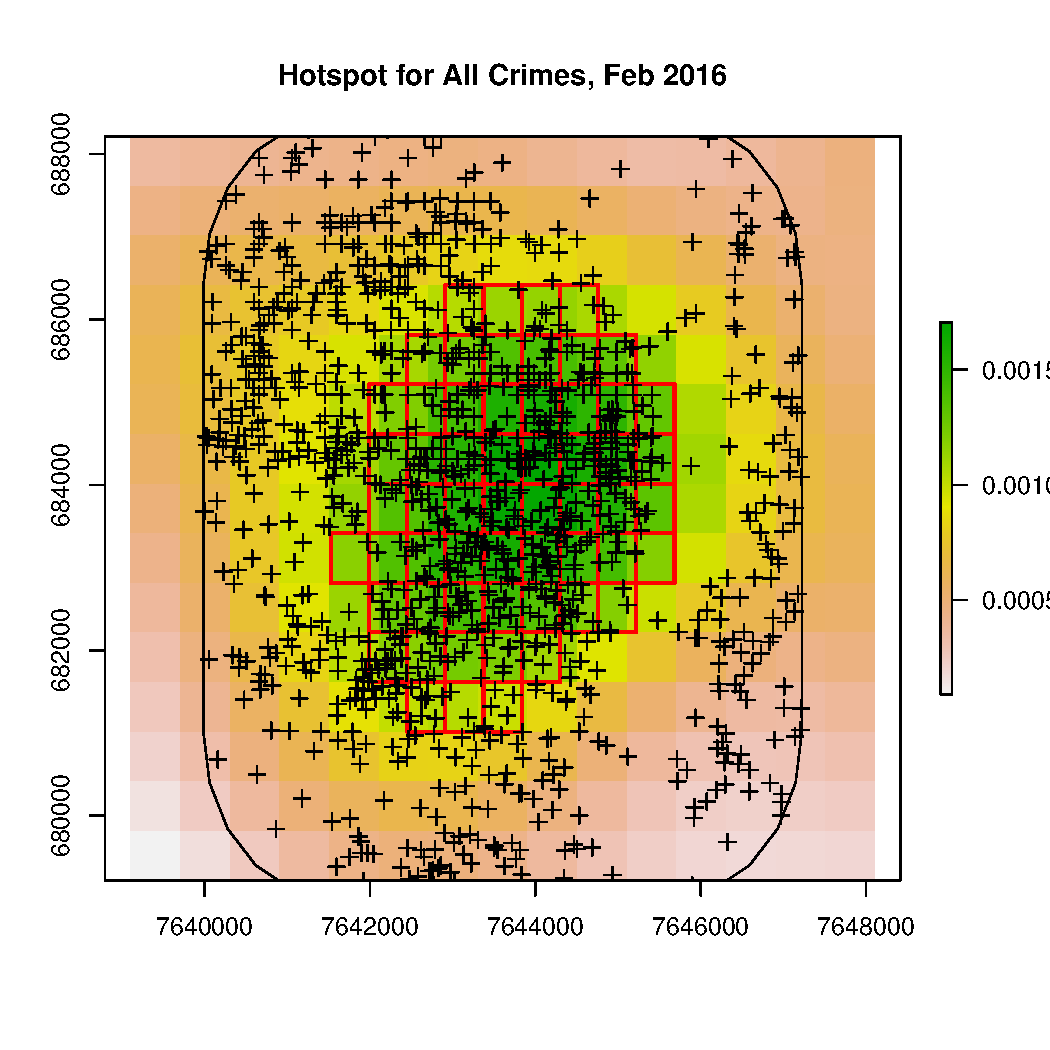
\includegraphics[scale=0.9]{figures/hotspot_all.pdf}
    \caption{Caption here}
    \label{fig:figure1}
\end{figure}

\end{document}